In task 3, the data files \texttt{nonlinear\_vectorfield\_data\_x0.txt} and \texttt{nonlinear\_vectorfield\_data\_x1.txt} are used. Both files display the same points. The first file contains the initial points, whereas the second dataset holds the points advanced with an evolution operator. A representation of that data can be found in Fig. \ref{fig:5-3} \\

\begin{figure}[H]
    \centering
    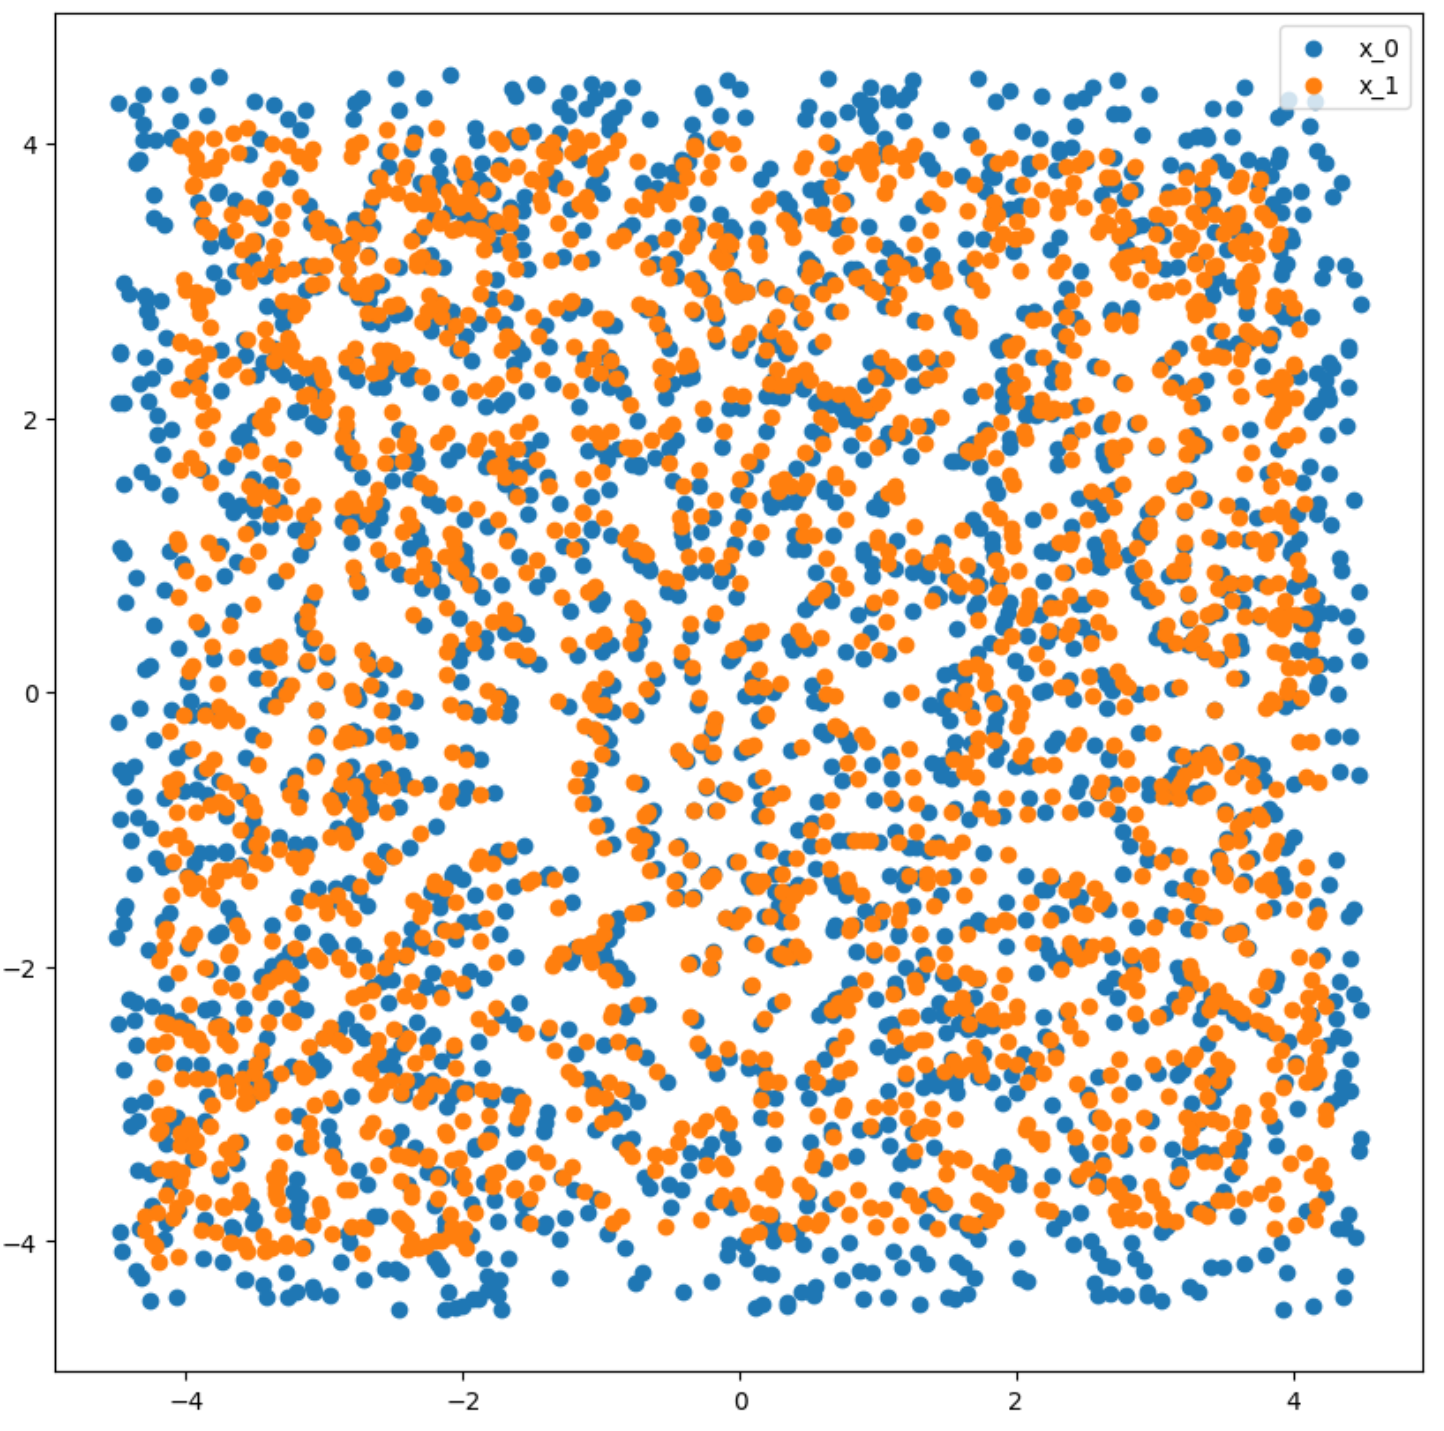
\includegraphics[width=0.4\linewidth]{images/5_3_data.png}
    \caption{Dataset for task 3}
    \label{fig:5-3}
\end{figure}

% Part 1: Estimate the vector field with a linear operator.
% Part 1: Compute the mean squared error to the solution after Δt as close as possible to x1.

\textbf{Part 1: Linear approximation} \\
In the first part of the task, a linear operator \texttt{A} needs to be estimated. This can be done similarly to task 2, using \texttt{lstsq} \cite{2020SciPy-NMeth}. However, we use a smaller $\Delta t$=0.01. Using the approximated \texttt{A} along with the function \texttt{linear\_approximation}, we can predict values $\hat{x_1}$. In Fig. \ref{fig:5-3-1a}, the predicted values are plotted against the original values $x_1$. It is evident that the linear approximation does not reflect the original values well. The image rather resembles $x_0$ and $x_1$ plotted against each other, indicating a weak approximation with almost no effect. The resulting Mean Squared Error (MSE) equals \texttt{0.0186}. \\


\begin{figure}[H]
\centering
    \begin{subfigure}{0.45\textwidth}
        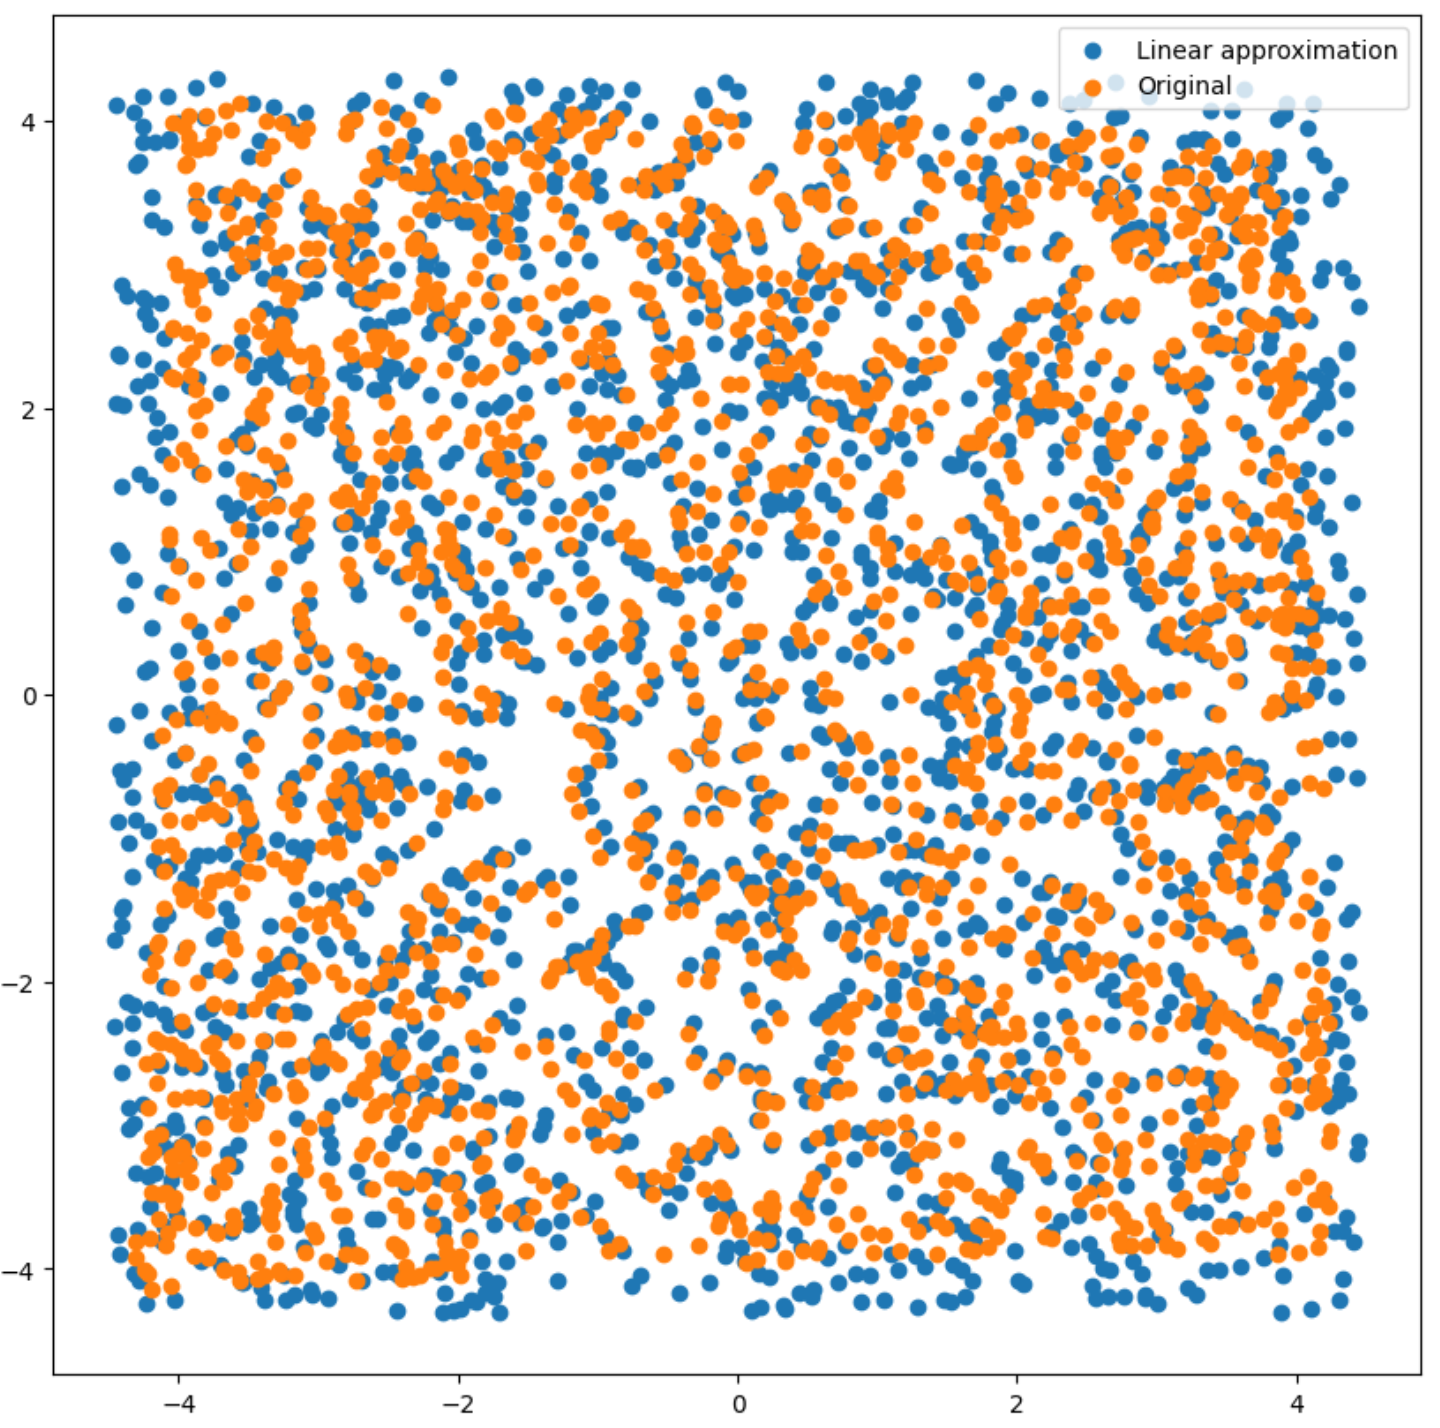
\includegraphics[width=\linewidth]{images/5_3_1_lin-approx.png}
        \caption{Linear approximation}
        \label{fig:5-3-1a}
    \end{subfigure}
    \begin{subfigure}{0.45\textwidth}
        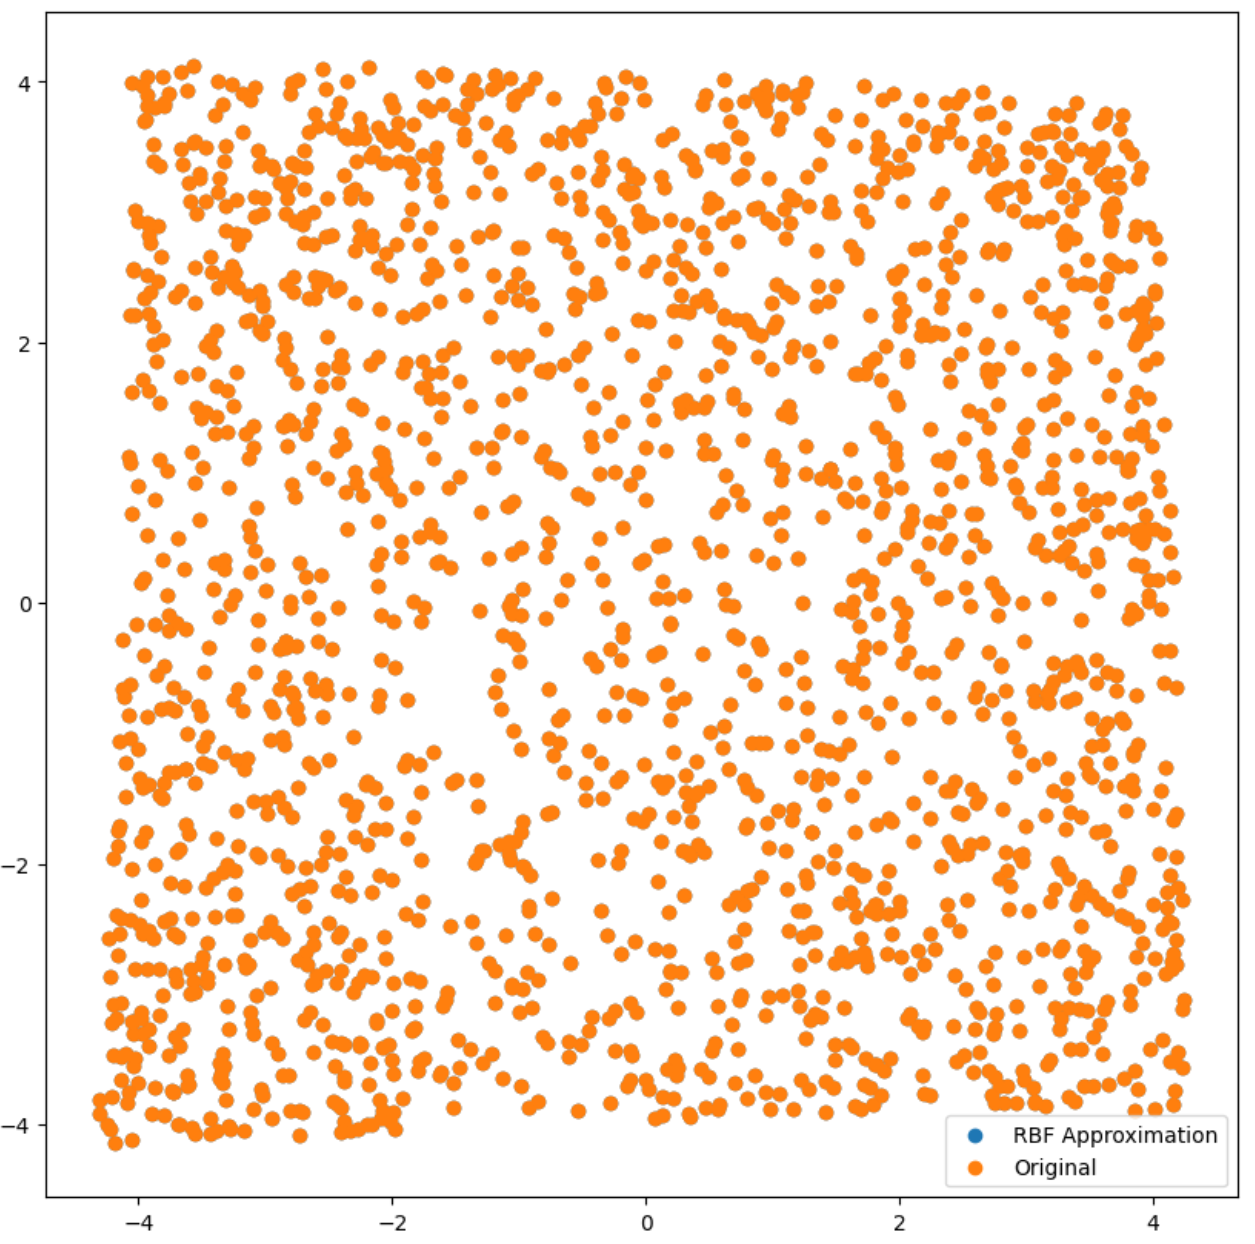
\includegraphics[width=\linewidth]{images/5_3_2_nonlin-approx.png}
        \caption{Nonlinear approximation}
        \label{fig:5-3-1b}
    \end{subfigure}
    \caption{$x_1$ plotted against $\hat{x_1}$}
    \label{fig:5-3-1}
\end{figure}

% Part 2: Approximate the vector field using radial basis functions.
% Part 2: How do the errors differ to the linear approximation?
% Part 2: What do you conclude: is the vector field linear or nonlinear? Why?

\textbf{Part 2: Nonlinear approximation} \\
To find the optimal MSE for RBF, we looped over multiple $l$ and $\epsilon$ values. The lowest \texttt{mse\_rbf} value was saved along with the values $l$ and $\epsilon$ that lead to this result: \\
\texttt{Least mean Squared Error (RBF): 2.898361613586458e-12 reached for: l=1000, eps=2} \\

Additionally, we plotted a graph to showcase how the $l$ and $\epsilon$ values affect the \texttt{mse\_rbf} outcome. This can be seen in Fig. \ref{fig:5-3-2}. The z-axis displays the resulting \texttt{mse\_rbf} values, which all are in the $e^{-12}$ range. 

\begin{figure}[H]
    \centering
    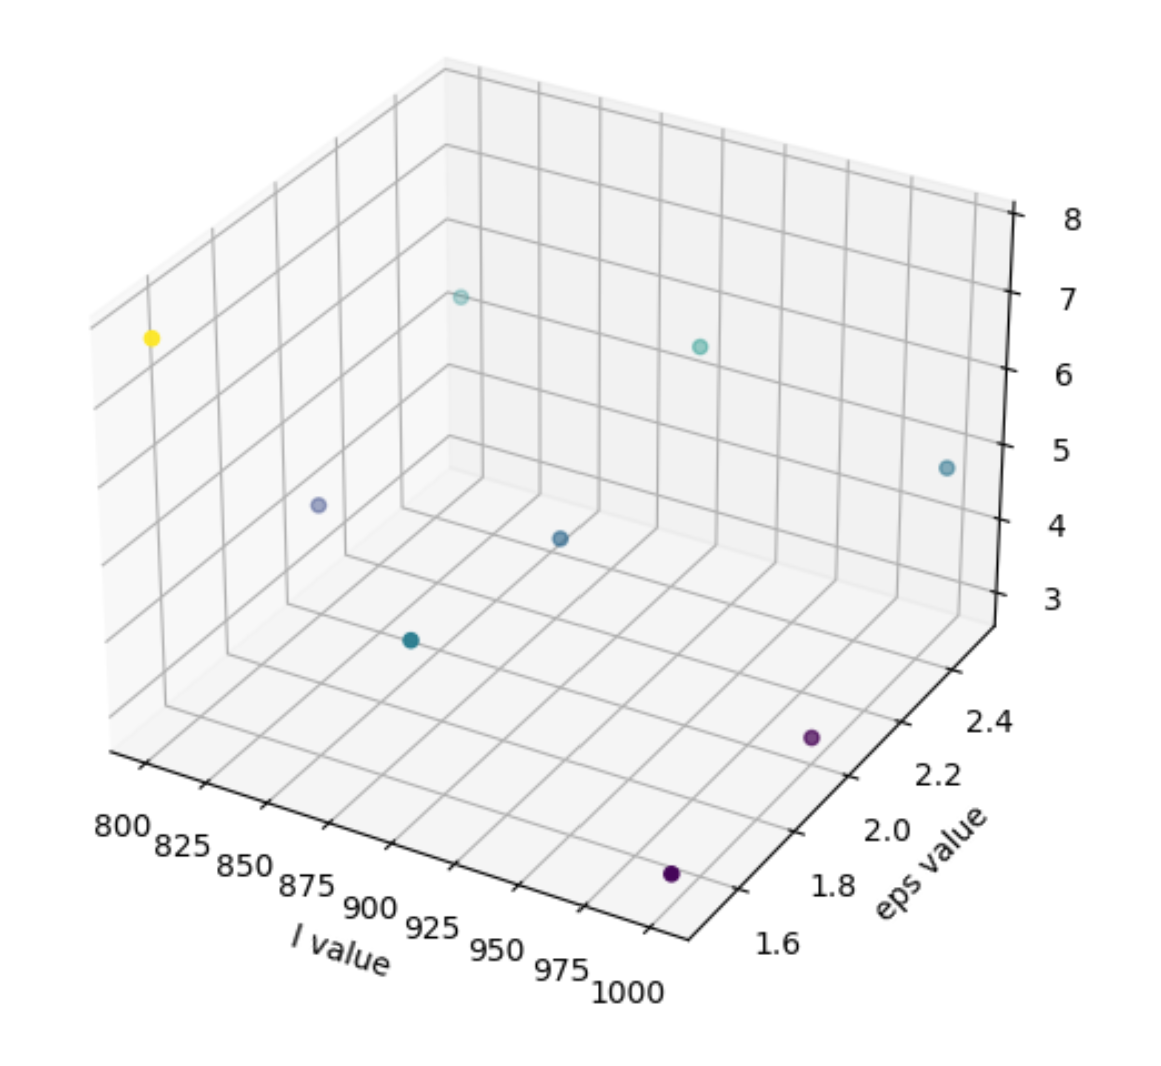
\includegraphics[width=0.5\linewidth]{images/5_3_2_value-comparison.png}
    \caption{Different $l$ and $\epsilon$ values with their resulting $mse\_rbf$ values}
    \label{fig:5-3-2}
\end{figure}

After the optimal values were evaluated, we employed them to calculate a second prediction using the function \texttt{nonlinear\_approximation}. The plotted result can be seen in Fig. \ref{fig:5-3-1b}. The approximated points lie virtually in the same position as the original $x_1$ values, indicating a very good prediction. \\ 

In comparison to linear approximation, the errors for RBF appear much smaller, down to values of $e^{-12}$. Therefore, it can be assumed that the vector field is nonlinear, just like the nonlinear approximation which yields better results. \\

% Part 3: Where do you end up, i.e. where are the steady states of the system?
% Part 3: Are there multiple steady states? Hint: yes, but less than 10.
% Part 3: Can the system be topologically equivalent to a linear system? Why (not)?

\textbf{Part 3: Steady States} \\
For the last part of task 3, we use nonlinear approximation since it proved to establish better predictions. Plotting the phase portrait results in Fig. \ref{fig:5-3-3}. Four points can be identified where the lines converge to. These points are the steady states of the system. 

\begin{figure}[H]
    \centering
    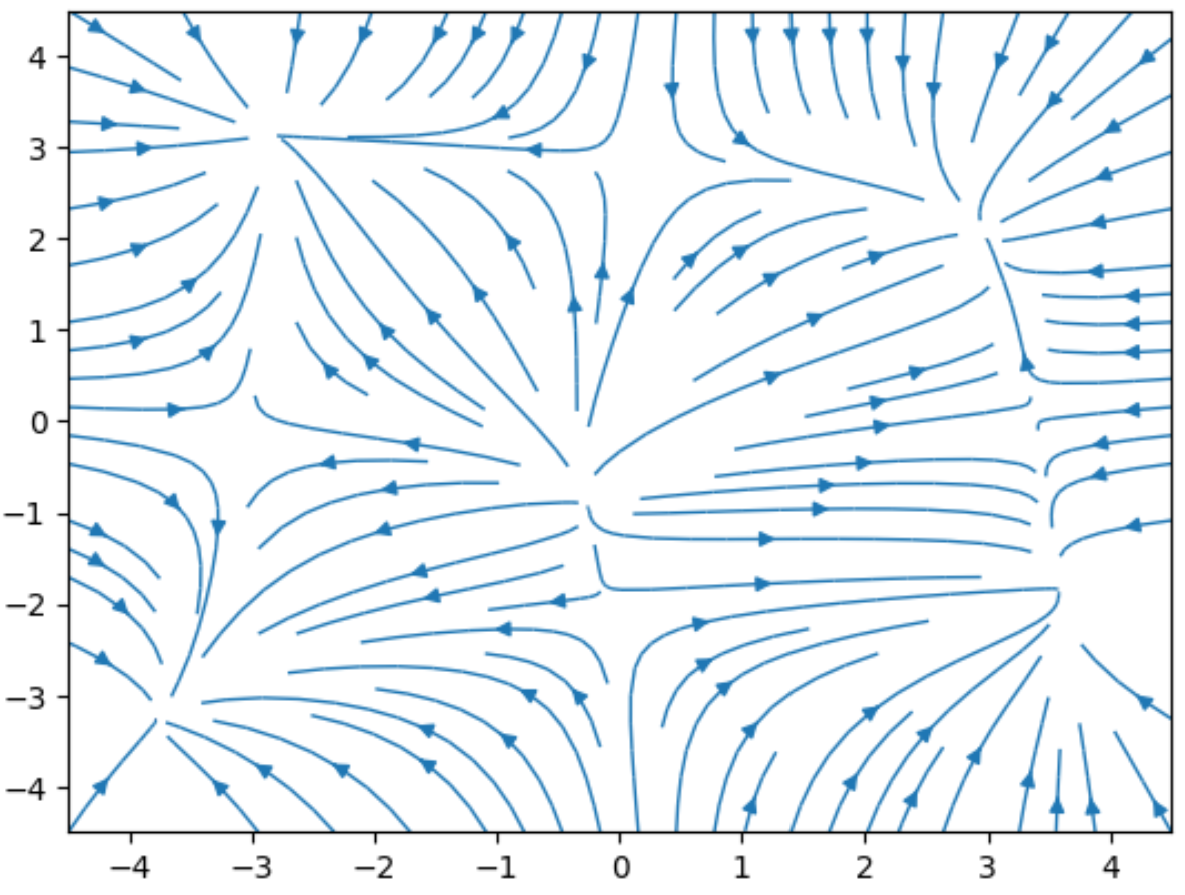
\includegraphics[width=0.7\linewidth]{images/5_3_3_phaseportrait-steadystates.png}
    \caption{Phase portrait depicting steady states}
    \label{fig:5-3-3}
\end{figure}

A linear system with a matrix A of size 2×2 can have 2 steady states at most. Therefore, the nonlinear approximated system cannot be topologically equivalent to a linear system. 

% Discussed how and why you chose the values of L and ϵ?